\documentclass{article}
\usepackage[utf8]{inputenc}

% Essential packages
\usepackage{amsmath, amssymb, amsfonts}
\usepackage{bm}
\usepackage{graphicx}
\usepackage{xcolor}
\usepackage{tcolorbox}
\usepackage{hyperref}
\usepackage{url}
\usepackage{booktabs}
\usepackage{array}
\usepackage{multirow}
\usepackage{enumitem}
\usepackage{tikz}
\usetikzlibrary{arrows.meta, positioning, shapes.geometric, matrix}

% Load conventions after math packages
\usepackage{../../shared/styles/conventions}

% Additional packages for tutorial format
\usepackage[margin=1in]{geometry}
\usepackage{fancyhdr}
\usepackage{titlesec}

% Header and footer setup
\pagestyle{fancy}
\fancyhf{}
\rhead{Tutorial 1: ML Conventions \& Metrics}
\lhead{ES335 - Machine Learning}
\rfoot{Page \thepage}

% Title formatting
\titleformat{\section}{\Large\bfseries\color{blue!75!black}}{\thesection}{1em}{}
\titleformat{\subsection}{\large\bfseries\color{blue!60!black}}{\thesubsection}{1em}{}

% Define counters
\newcounter{example}
\setcounter{example}{0}
\newcounter{exercise}
\setcounter{exercise}{0}

\title{\textbf{Tutorial 1: Machine Learning Conventions and Evaluation Metrics} \\ \textit{From Mathematical Notation to Performance Assessment}}
\author{ES335 - Machine Learning \\ IIT Gandhinagar}
\date{\today}

\begin{document}

\maketitle

\begin{abstract}
This tutorial bridges mathematical foundations with practical machine learning. We establish standard notation conventions used throughout ML literature, then dive deep into evaluation metrics for classification and regression. Through real-world examples and comprehensive exercises, you'll learn not just what these metrics mean mathematically, but when and why to use them in practice.
\end{abstract}

\tableofcontents
\newpage

\section{Introduction: From Math to Machine Learning}

In Tutorial 0, you learned the mathematical building blocks. Now we'll see how these concepts come alive in machine learning:

\begin{itemize}
    \item \textbf{Datasets} become matrices where each row is a sample
    \item \textbf{Features} become columns in our data matrix  
    \item \textbf{Predictions} are vectors comparing our model to reality
    \item \textbf{Performance} is measured using mathematical functions of these comparisons
\end{itemize}

Think of this tutorial as learning the "language" of machine learning - both the notation and the vocabulary for measuring success.

\section{Standard ML Notation and Conventions}

\subsection{Dataset Representation}

The foundation of any ML problem starts with data representation:

\begin{center}
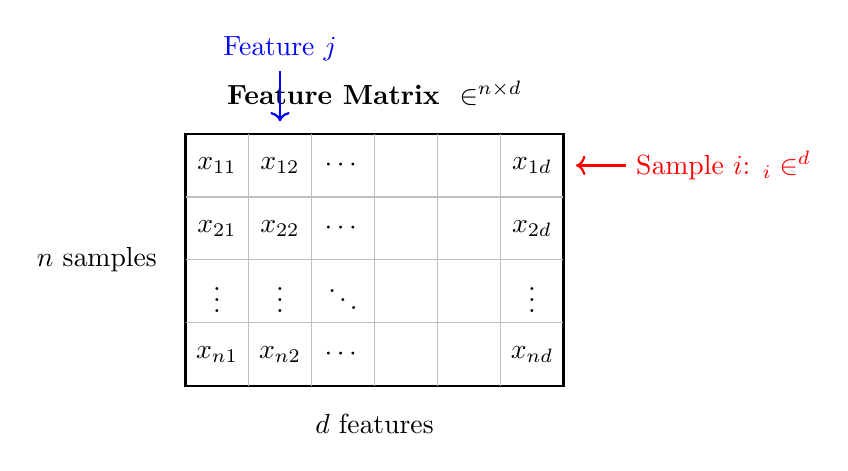
\begin{tikzpicture}[scale=0.8]
    % Draw the data matrix
    \draw[thick] (0,0) rectangle (6,4);
    
    % Draw grid lines
    \foreach \x in {1,2,3,4,5} \draw[gray!50] (\x,0) -- (\x,4);
    \foreach \y in {1,2,3} \draw[gray!50] (0,\y) -- (6,\y);
    
    % Labels
    \node[above] at (3,4.3) {\textbf{Feature Matrix } $\mX \in \Real^{n \times d}$};
    \node[left] at (-0.3,2) {$n$ samples};
    \node[below] at (3,-0.3) {$d$ features};
    
    % Sample entries
    \node at (0.5,3.5) {$x_{11}$};
    \node at (1.5,3.5) {$x_{12}$};
    \node at (2.5,3.5) {$\cdots$};
    \node at (5.5,3.5) {$x_{1d}$};
    \node at (0.5,2.5) {$x_{21}$};
    \node at (1.5,2.5) {$x_{22}$};
    \node at (2.5,2.5) {$\cdots$};
    \node at (5.5,2.5) {$x_{2d}$};
    \node at (0.5,1.5) {$\vdots$};
    \node at (1.5,1.5) {$\vdots$};
    \node at (2.5,1.5) {$\ddots$};
    \node at (5.5,1.5) {$\vdots$};
    \node at (0.5,0.5) {$x_{n1}$};
    \node at (1.5,0.5) {$x_{n2}$};
    \node at (2.5,0.5) {$\cdots$};
    \node at (5.5,0.5) {$x_{nd}$};
    
    % Arrow pointing to row
    \draw[->, thick, red] (7,3.5) -- (6.2,3.5);
    \node[red, right] at (7,3.5) {Sample $i$: $\vx_i \in \Real^d$};
    
    % Arrow pointing to column  
    \draw[->, thick, blue] (1.5,5) -- (1.5,4.2);
    \node[blue, above] at (1.5,5) {Feature $j$};
\end{tikzpicture}
\end{center}

\textbf{Key Conventions}:
\begin{itemize}
    \item $\mX \in \Real^{n \times d}$: Feature matrix (rows = samples, columns = features)
    \item $\vx_i \in \Real^d$: $i$-th sample (row vector)
    \item $\vy \in \Real^n$: Target vector (column vector)
    \item $\hat{\vy} \in \Real^n$: Predictions vector
    \item $\cD = \{(\vx_i, y_i)\}_{i=1}^n$: Dataset as collection of (input, output) pairs
\end{itemize}

\begin{tcolorbox}[colback=blue!5!white,colframe=blue!75!black,title=Example \stepcounter{example}\#\theexample: House Price Dataset]
Predicting house prices using 3 features for 4 houses:

$$\mX = \begin{bmatrix} 
1850 & 3 & 25 \\
2200 & 4 & 10 \\
1200 & 2 & 35 \\
2800 & 5 & 8
\end{bmatrix}, \quad \vy = \begin{bmatrix} 
425000 \\
520000 \\
280000 \\
750000
\end{bmatrix}$$

Where columns represent: [Square Feet, Bedrooms, Age in Years]

Here: $n = 4$ houses, $d = 3$ features
- $\vx_1 = [1850, 3, 25]^T$ (first house)
- $y_1 = 425000$ (first house price)
\end{tcolorbox}

\subsection{Model Notation}

\textbf{Hypothesis/Model Function}: $f: \Real^d \rightarrow \Real$ (regression) or $f: \Real^d \rightarrow \{1,2,\ldots,k\}$ (classification)

\textbf{Parametric Models}: $f(\vx; \vtheta)$ where $\vtheta$ are learnable parameters
\begin{itemize}
    \item Linear regression: $f(\vx; \vw, b) = \vw^T \vx + b$
    \item Logistic regression: $f(\vx; \vw, b) = \sigma(\vw^T \vx + b)$
    \item Neural network: $f(\vx; \Theta) = \text{NN}(\vx; \Theta)$
\end{itemize}

\textbf{Training Process}:
$$\vtheta^* = \arg\min_{\vtheta} \frac{1}{n} \sum_{i=1}^n L(f(\vx_i; \vtheta), y_i)$$

where $L(\cdot, \cdot)$ is a loss function.

\subsection{Probability Notation in ML}

\textbf{Discriminative Models}: $P(y|\vx)$ - probability of output given input
\textbf{Generative Models}: $P(\vx|y)$ - probability of input given output

\textbf{Classification Probabilities}:
\begin{itemize}
    \item Binary: $P(y=1|\vx), P(y=0|\vx)$ where $P(y=1|\vx) + P(y=0|\vx) = 1$
    \item Multiclass: $P(y=c|\vx)$ for $c \in \{1,2,\ldots,k\}$, where $\sum_{c=1}^k P(y=c|\vx) = 1$
\end{itemize}

\section{Classification Metrics: Measuring Success}

\subsection{The Foundation: Confusion Matrix}

Before diving into metrics, let's understand the confusion matrix - the source of all classification metrics:

\begin{center}
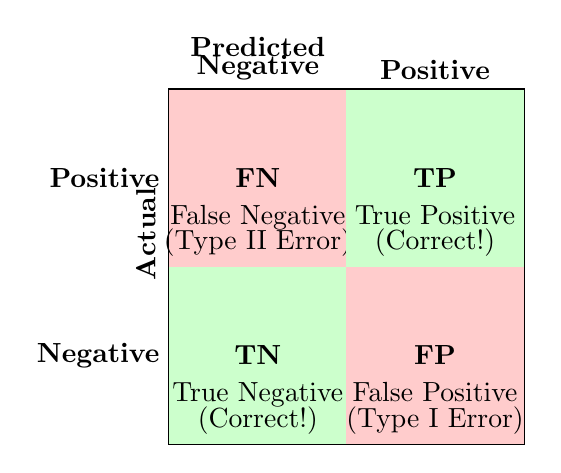
\begin{tikzpicture}[scale=1.5]
    % Draw confusion matrix
    \draw[thick] (0,0) rectangle (3,3);
    \draw[thick] (1.5,0) -- (1.5,3);
    \draw[thick] (0,1.5) -- (3,1.5);
    
    % Labels
    \node[above] at (0.75,3.2) {\textbf{Predicted}};
    \node[above] at (0.75,3) {\textbf{Negative}};
    \node[above] at (2.25,3) {\textbf{Positive}};
    
    \node[left, rotate=90] at (-0.2,2.25) {\textbf{Actual}};
    \node[left] at (0,2.25) {\textbf{Positive}};
    \node[left] at (0,0.75) {\textbf{Negative}};
    
    % Fill cells
    \fill[red!20] (0,1.5) rectangle (1.5,3);
    \node at (0.75,2.25) {\textbf{FN}};
    \node[below] at (0.75,2.1) {False Negative};
    \node[below] at (0.75,1.9) {(Type II Error)};
    
    \fill[green!20] (1.5,1.5) rectangle (3,3);
    \node at (2.25,2.25) {\textbf{TP}};
    \node[below] at (2.25,2.1) {True Positive};
    \node[below] at (2.25,1.9) {(Correct!)};
    
    \fill[red!20] (1.5,0) rectangle (3,1.5);
    \node at (2.25,0.75) {\textbf{FP}};
    \node[below] at (2.25,0.6) {False Positive};
    \node[below] at (2.25,0.4) {(Type I Error)};
    
    \fill[green!20] (0,0) rectangle (1.5,1.5);
    \node at (0.75,0.75) {\textbf{TN}};
    \node[below] at (0.75,0.6) {True Negative};
    \node[below] at (0.75,0.4) {(Correct!)};
\end{tikzpicture}
\end{center}

\begin{tcolorbox}[colback=orange!5!white,colframe=orange!75!black,title=Example \stepcounter{example}\#\theexample: Email Spam Detection]
Your spam filter processed 1000 emails with these results:

\begin{center}
\begin{tabular}{|c|c|c|}
\hline
& \textbf{Predicted Not Spam} & \textbf{Predicted Spam} \\
\hline
\textbf{Actually Not Spam} & 850 (TN) & 50 (FP) \\
\hline
\textbf{Actually Spam} & 20 (FN) & 80 (TP) \\
\hline
\end{tabular}
\end{center}

From this confusion matrix, we can calculate all classification metrics:
- Total emails: 1000
- Correct predictions: 850 + 80 = 930
- Incorrect predictions: 50 + 20 = 70
\end{tcolorbox}

\subsection{Core Classification Metrics}

\textbf{1. Accuracy}: Overall correctness
$$\text{Accuracy} = \frac{TP + TN}{TP + TN + FP + FN} = \frac{\text{Correct Predictions}}{\text{Total Predictions}}$$

\textbf{2. Precision}: Of predicted positives, how many were correct?
$$\text{Precision} = \frac{TP}{TP + FP} = \frac{\text{True Positives}}{\text{Predicted Positives}}$$

\textbf{3. Recall (Sensitivity)}: Of actual positives, how many did we find?
$$\text{Recall} = \frac{TP}{TP + FN} = \frac{\text{True Positives}}{\text{Actual Positives}}$$

\textbf{4. Specificity}: Of actual negatives, how many did we correctly identify?
$$\text{Specificity} = \frac{TN}{TN + FP} = \frac{\text{True Negatives}}{\text{Actual Negatives}}$$

\textbf{5. F1-Score}: Harmonic mean of precision and recall
$$F_1 = \frac{2 \times \text{Precision} \times \text{Recall}}{\text{Precision} + \text{Recall}} = \frac{2 \times TP}{2 \times TP + FP + FN}$$

\begin{center}
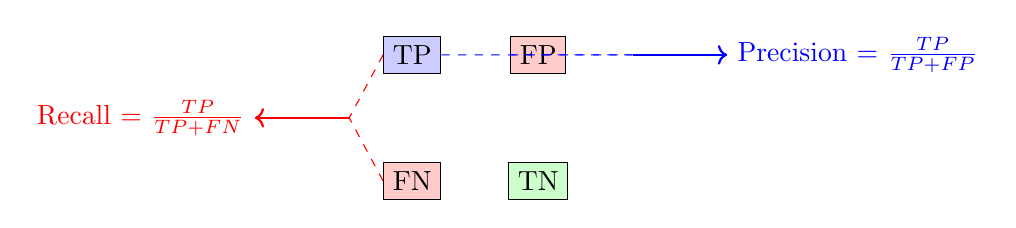
\begin{tikzpicture}[scale=0.8]
    % Draw metric relationships
    \node[rectangle, draw, fill=blue!20] (tp) at (0,2) {TP};
    \node[rectangle, draw, fill=red!20] (fp) at (2,2) {FP};
    \node[rectangle, draw, fill=red!20] (fn) at (0,0) {FN};
    \node[rectangle, draw, fill=green!20] (tn) at (2,0) {TN};
    
    % Precision arrow
    \draw[->, thick, blue] (3.5,2) -- (5,2) node[right] {Precision = $\frac{TP}{TP + FP}$};
    \draw[blue, dashed] (tp.east) -- (3.5,2);
    \draw[blue, dashed] (fp.west) -- (3.5,2);
    
    % Recall arrow
    \draw[->, thick, red] (-1,1) -- (-2.5,1) node[left] {Recall = $\frac{TP}{TP + FN}$};
    \draw[red, dashed] (tp.west) -- (-1,1);
    \draw[red, dashed] (fn.west) -- (-1,1);
\end{tikzpicture}
\end{center}

\subsection{When to Use Which Metric?}

Understanding when each metric is appropriate is crucial:

\begin{tcolorbox}[colback=yellow!5!white,colframe=yellow!75!black,title=Example \stepcounter{example}\#\theexample: Medical Diagnosis - Cancer Detection]
Context: Screening 10,000 people for a rare cancer (1\% prevalence)

\textbf{Scenario 1: Conservative Model}
- TP: 90, FP: 100, FN: 10, TN: 9800
- Accuracy: 98.9\% (looks great!)
- Precision: 47.4\% (only half of positive predictions are correct)
- Recall: 90\% (finds most cancer cases)

\textbf{Why accuracy is misleading}: With 99\% healthy people, a model that always predicts "healthy" would get 99\% accuracy!

\textbf{What matters here}:
- \textbf{Recall} is critical (can't miss cancer cases)
- \textbf{Precision} is important (too many false alarms waste resources)
- \textbf{F1-score} balances both concerns
\end{tcolorbox}

\begin{tcolorbox}[colback=cyan!5!white,colframe=cyan!75!black,title=Example \stepcounter{example}\#\theexample: Information Retrieval - Search Engine]
Context: Search results for "machine learning courses"

\textbf{User's Perspective}:
- \textbf{Precision matters most}: First 10 results should be relevant
- \textbf{Recall less critical}: User won't scroll through 1000s of results

\textbf{Search Engine's Perspective}:
- \textbf{Precision}: Satisfied users return
- \textbf{Recall}: Comprehensive coverage builds trust
- \textbf{Balance}: Precision@K (precision of top K results)
\end{tcolorbox}

\subsection{Advanced Classification Metrics}

\textbf{ROC Curve}: Plots True Positive Rate vs False Positive Rate
- TPR = Recall = $\frac{TP}{TP + FN}$  
- FPR = $\frac{FP}{FP + TN}$ (1 - Specificity)

\textbf{AUC-ROC}: Area Under ROC Curve
- AUC = 1.0: Perfect classifier
- AUC = 0.5: Random classifier
- AUC = 0.0: Perfectly wrong classifier (flip predictions!)

\textbf{Precision-Recall Curve}: Especially useful for imbalanced datasets

\begin{center}
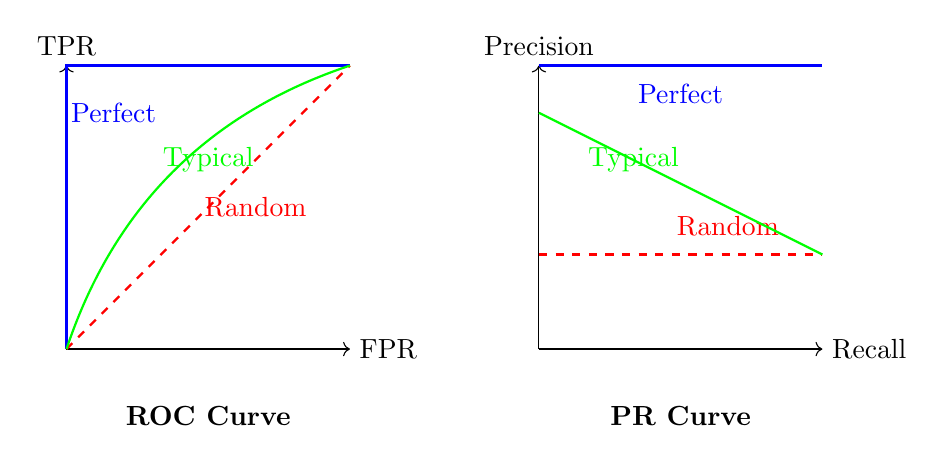
\begin{tikzpicture}[scale=1.2]
    % ROC Curve
    \begin{scope}[shift={(0,0)}]
        \draw[->] (0,0) -- (3,0) node[right] {FPR};
        \draw[->] (0,0) -- (0,3) node[above] {TPR};
        
        % Perfect classifier
        \draw[thick, blue] (0,0) -- (0,3) -- (3,3);
        \node[blue] at (0.5,2.5) {Perfect};
        
        % Random classifier
        \draw[thick, red, dashed] (0,0) -- (3,3);
        \node[red] at (2,1.5) {Random};
        
        % Realistic classifier
        \draw[thick, green] (0,0) .. controls (0.5,1.5) and (1.5,2.5) .. (3,3);
        \node[green] at (1.5,2) {Typical};
        
        \node[below] at (1.5,-0.5) {\textbf{ROC Curve}};
    \end{scope}
    
    % PR Curve
    \begin{scope}[shift={(5,0)}]
        \draw[->] (0,0) -- (3,0) node[right] {Recall};
        \draw[->] (0,0) -- (0,3) node[above] {Precision};
        
        % Perfect classifier
        \draw[thick, blue] (0,3) -- (3,3);
        \node[blue] at (1.5,2.7) {Perfect};
        
        % Random classifier (depends on class balance)
        \draw[thick, red, dashed] (0,1) -- (3,1);
        \node[red] at (2,1.3) {Random};
        
        % Realistic classifier
        \draw[thick, green] (0,2.5) .. controls (1,2) and (2,1.5) .. (3,1);
        \node[green] at (1,2) {Typical};
        
        \node[below] at (1.5,-0.5) {\textbf{PR Curve}};
    \end{scope}
\end{tikzpicture}
\end{center}

\section{Regression Metrics: Measuring Continuous Predictions}

When predicting continuous values (house prices, temperatures, stock prices), we need different metrics:

\subsection{Core Regression Metrics}

\textbf{1. Mean Absolute Error (MAE)}:
$$\text{MAE} = \frac{1}{n} \sum_{i=1}^n |y_i - \hat{y}_i|$$

- Interpretable: Same units as target variable
- Robust to outliers
- All errors weighted equally

\textbf{2. Mean Squared Error (MSE)}:
$$\text{MSE} = \frac{1}{n} \sum_{i=1}^n (y_i - \hat{y}_i)^2$$

- Penalizes large errors more heavily
- Differentiable (useful for optimization)
- Units are squared

\textbf{3. Root Mean Squared Error (RMSE)}:
$$\text{RMSE} = \sqrt{\text{MSE}} = \sqrt{\frac{1}{n} \sum_{i=1}^n (y_i - \hat{y}_i)^2}$$

- Same units as target variable
- Still penalizes large errors
- Most commonly reported

\textbf{4. Mean Absolute Percentage Error (MAPE)}:
$$\text{MAPE} = \frac{100\%}{n} \sum_{i=1}^n \left|\frac{y_i - \hat{y}_i}{y_i}\right|$$

- Scale-independent (percentage)
- Interpretable across different problems
- Problems when $y_i$ is near zero

\textbf{5. R-squared (Coefficient of Determination)}:
$$R^2 = 1 - \frac{\text{SS}_{\text{res}}}{\text{SS}_{\text{tot}}} = 1 - \frac{\sum_{i=1}^n (y_i - \hat{y}_i)^2}{\sum_{i=1}^n (y_i - \bar{y})^2}$$

where $\bar{y} = \frac{1}{n}\sum_{i=1}^n y_i$ is the mean of actual values.

- $R^2 = 1$: Perfect predictions
- $R^2 = 0$: Model as good as predicting the mean
- $R^2 < 0$: Model worse than predicting the mean

\begin{tcolorbox}[colback=purple!5!white,colframe=purple!75!black,title=Example \stepcounter{example}\#\theexample: House Price Prediction Comparison]
Two models predicting house prices (in thousands):

\textbf{Actual prices}: [300, 450, 280, 520, 380]\\
\textbf{Model A}: [310, 440, 290, 510, 370] (conservative)\\
\textbf{Model B}: [280, 500, 260, 550, 400] (more variable)

\textbf{Model A Metrics}:
- MAE: $\frac{|10|+|10|+|10|+|10|+|10|}{5} = 10$ thousand
- MSE: $\frac{10^2+10^2+10^2+10^2+10^2}{5} = 100$
- RMSE: $\sqrt{100} = 10$ thousand

\textbf{Model B Metrics}:
- MAE: $\frac{|20|+|50|+|20|+|30|+|20|}{5} = 28$ thousand
- MSE: $\frac{20^2+50^2+20^2+30^2+20^2}{5} = 780$
- RMSE: $\sqrt{780} = 27.9$ thousand

Model A is better on all metrics, especially RMSE which penalizes the large \$50k error in Model B.
\end{tcolorbox}

\subsection{Choosing the Right Regression Metric}

\begin{center}
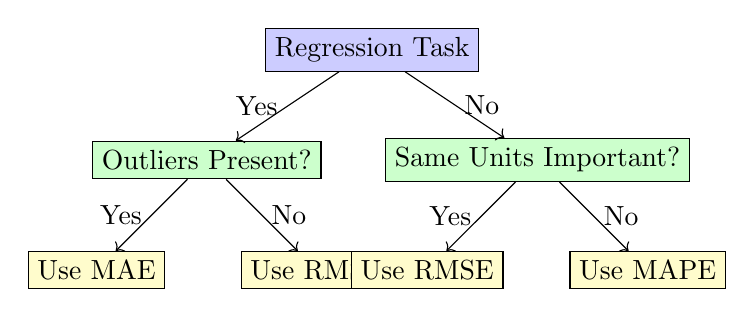
\begin{tikzpicture}[scale=0.7]
    % Create decision tree for metric selection
    \node[rectangle, draw, fill=blue!20] (root) at (0,0) {Regression Task};
    
    \node[rectangle, draw, fill=green!20] (outliers) at (-3,-2) {Outliers Present?};
    \node[rectangle, draw, fill=green!20] (units) at (3,-2) {Same Units Important?};
    
    \node[rectangle, draw, fill=yellow!20] (mae) at (-5,-4) {Use MAE};
    \node[rectangle, draw, fill=yellow!20] (rmse1) at (-1,-4) {Use RMSE};
    \node[rectangle, draw, fill=yellow!20] (rmse2) at (1,-4) {Use RMSE};
    \node[rectangle, draw, fill=yellow!20] (mape) at (5,-4) {Use MAPE};
    
    % Draw connections
    \draw[->] (root) -- (outliers) node[midway, left] {Yes};
    \draw[->] (root) -- (units) node[midway, right] {No};
    
    \draw[->] (outliers) -- (mae) node[midway, left] {Yes};
    \draw[->] (outliers) -- (rmse1) node[midway, right] {No};
    
    \draw[->] (units) -- (rmse2) node[midway, left] {Yes};
    \draw[->] (units) -- (mape) node[midway, right] {No};
\end{tikzpicture}
\end{center}

\section{Multiclass Classification}

Real-world classification often involves more than two classes:

\subsection{Extending Binary Metrics}

\textbf{Macro Averaging}: Calculate metric for each class, then average
$$\text{Macro-}F_1 = \frac{1}{k} \sum_{c=1}^k F_{1,c}$$

\textbf{Micro Averaging}: Pool all predictions, then calculate metric
$$\text{Micro-}F_1 = \frac{2 \times \sum_{c=1}^k TP_c}{2 \times \sum_{c=1}^k TP_c + \sum_{c=1}^k FP_c + \sum_{c=1}^k FN_c}$$

\textbf{Weighted Averaging}: Weight by class frequency
$$\text{Weighted-}F_1 = \sum_{c=1}^k \frac{n_c}{n} F_{1,c}$$

where $n_c$ is the number of samples in class $c$.

\begin{tcolorbox}[colback=teal!5!white,colframe=teal!75!black,title=Example \stepcounter{example}\#\theexample: Image Classification (3 classes)]
Confusion matrix for classifying images into [Dog, Cat, Bird]:

\begin{center}
\begin{tabular}{|c|c|c|c|}
\hline
& \textbf{Pred Dog} & \textbf{Pred Cat} & \textbf{Pred Bird} \\
\hline
\textbf{Actual Dog} & 85 & 10 & 5 \\
\hline
\textbf{Actual Cat} & 15 & 75 & 10 \\
\hline
\textbf{Actual Bird} & 8 & 12 & 80 \\
\hline
\end{tabular}
\end{center}

\textbf{Per-class metrics}:
- Dog: Precision = 85/(85+15+8) = 78.7\%, Recall = 85/100 = 85\%
- Cat: Precision = 75/(10+75+12) = 77.3\%, Recall = 75/100 = 75\%  
- Bird: Precision = 80/(5+10+80) = 84.2\%, Recall = 80/100 = 80\%

\textbf{Macro-F1}: Average of individual class F1 scores\\
\textbf{Micro-F1}: Based on total TP, FP, FN across all classes
\end{tcolorbox}

\section{Cross-Validation and Evaluation Best Practices}

\subsection{Why Standard Train/Test Split Isn't Enough}

\begin{itemize}
    \item Results depend on the particular split chosen
    \item May not use all data effectively
    \item Hard to tune hyperparameters without overfitting
    \item No confidence intervals on performance
\end{itemize}

\subsection{K-Fold Cross-Validation}

\begin{center}
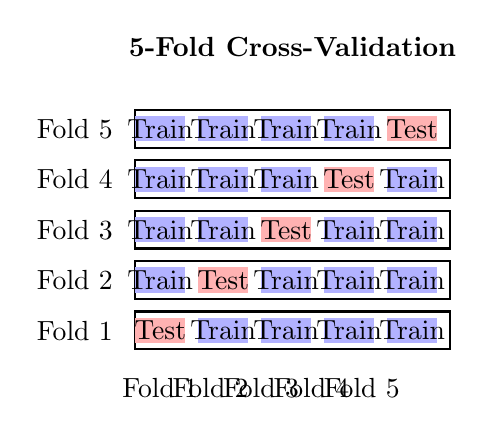
\begin{tikzpicture}[scale=0.8]
    % Draw 5-fold CV visualization
    \foreach \i in {0,1,2,3,4} {
        \draw[thick] (0,\i*0.8) rectangle (5,\i*0.8+0.6);
        
        % Color the folds
        \foreach \j in {0,1,2,3,4} {
            \pgfmathsetmacro{\x}{\j}
            \pgfmathsetmacro{\y}{\i*0.8+0.1}
            \pgfmathsetmacro{\w}{0.8}
            \pgfmathsetmacro{\h}{0.4}
            
            \ifnum\i=\j
                \fill[red!30] (\x,\y) rectangle (\x+\w,\y+\h);
                \node at (\x+\w/2,\y+\h/2) {Test};
            \else
                \fill[blue!30] (\x,\y) rectangle (\x+\w,\y+\h);
                \node at (\x+\w/2,\y+\h/2) {Train};
            \fi
        }
        
        \node[left] at (-0.2,\i*0.8+0.3) {Fold \pgfmathparse{int(\i+1)}\pgfmathresult};
    }
    
    \node[above] at (2.5,4.5) {\textbf{5-Fold Cross-Validation}};
    \node[below] at (0.4,-0.3) {Fold 1};
    \node[below] at (1.2,-0.3) {Fold 2};
    \node[below] at (2.0,-0.3) {Fold 3};
    \node[below] at (2.8,-0.3) {Fold 4};
    \node[below] at (3.6,-0.3) {Fold 5};
\end{tikzpicture}
\end{center}

\textbf{Process}:
1. Split data into $k$ equal folds
2. For each fold $i$:
   - Train on remaining $k-1$ folds
   - Test on fold $i$
   - Record performance metric
3. Report mean and standard deviation of metric

\textbf{Benefits}:
- Every sample used for both training and testing
- More robust performance estimates
- Confidence intervals via standard deviation
- Better hyperparameter tuning

\section{Common Pitfalls and Best Practices}

\subsection{Data Leakage}

\textbf{What is data leakage?} Information from the test set influences the training process.

\textbf{Common forms}:
\begin{itemize}
    \item Preprocessing on entire dataset before splitting
    \item Feature selection using entire dataset
    \item Hyperparameter tuning using test set
    \item Temporal leakage in time series
\end{itemize}

\begin{tcolorbox}[colback=red!5!white,colframe=red!75!black,title=Example \stepcounter{example}\#\theexample: Preprocessing Data Leakage]
\textbf{WRONG}: 
\begin{enumerate}
    \item Normalize entire dataset: $X_{normalized} = \frac{X - \mu_{all}}{\sigma_{all}}$
    \item Split into train/test
    \item Train model on normalized train set
    \item Test on normalized test set
\end{enumerate}

\textbf{Problem}: Test set statistics influenced the training data!

\textbf{CORRECT}:
\begin{enumerate}
    \item Split into train/test
    \item Normalize training set: $X_{train,norm} = \frac{X_{train} - \mu_{train}}{\sigma_{train}}$
    \item Normalize test set using training stats: $X_{test,norm} = \frac{X_{test} - \mu_{train}}{\sigma_{train}}$
    \item Train and test on respective normalized sets
\end{enumerate}
\end{tcolorbox}

\subsection{Class Imbalance}

When classes are severely imbalanced (e.g., 99\% vs 1\%), accuracy becomes misleading.

\textbf{Solutions}:
\begin{itemize}
    \item Use precision, recall, F1-score instead of accuracy
    \item Stratified sampling in cross-validation
    \item Class weighting in loss functions
    \item Resampling techniques (SMOTE, undersampling)
    \item Different probability thresholds
\end{itemize}

\subsection{Multiple Comparisons Problem}

When testing many models/hyperparameters, some will appear good by chance.

\textbf{Solutions}:
\begin{itemize}
    \item Hold-out validation set separate from test set
    \item Bonferroni correction for p-values
    \item Nested cross-validation
    \item Report confidence intervals
\end{itemize}

\section{Practice Problems}

\subsection{Warm-up Problems}

\begin{tcolorbox}[colback=gray!5!white,colframe=gray!75!black,title=Problem \stepcounter{exercise}\#\theexercise: Confusion Matrix Calculations]
A binary classifier produces this confusion matrix:

\begin{center}
\begin{tabular}{|c|c|c|}
\hline
& \textbf{Predicted 0} & \textbf{Predicted 1} \\
\hline
\textbf{Actual 0} & 850 & 50 \\
\hline
\textbf{Actual 1} & 100 & 200 \\
\hline
\end{tabular}
\end{center}

Calculate: (a) Accuracy, (b) Precision, (c) Recall, (d) Specificity, (e) F1-score

\textbf{Solutions}:
- TP=200, TN=850, FP=50, FN=100
- (a) Accuracy = (200+850)/1200 = 87.5\%
- (b) Precision = 200/(200+50) = 80\%  
- (c) Recall = 200/(200+100) = 66.7\%
- (d) Specificity = 850/(850+50) = 94.4\%
- (e) F1 = 2×(0.8×0.667)/(0.8+0.667) = 72.7\%
\end{tcolorbox}

\begin{tcolorbox}[colback=gray!5!white,colframe=gray!75!black,title=Problem \stepcounter{exercise}\#\theexercise: Regression Metrics]
Given predictions and actual values:
- Actual: [100, 150, 200, 250, 300]
- Predicted: [110, 140, 190, 260, 290]

Calculate: (a) MAE, (b) MSE, (c) RMSE, (d) MAPE

\textbf{Solutions}:
- Errors: [10, -10, -10, 10, -10]
- (a) MAE = (10+10+10+10+10)/5 = 10
- (b) MSE = (100+100+100+100+100)/5 = 100  
- (c) RMSE = $\sqrt{100}$ = 10
- (d) MAPE = (10/100 + 10/150 + 10/200 + 10/250 + 10/300)/5 × 100 = 6.33\%
\end{tcolorbox}

\subsection{Intermediate Problems}

\begin{tcolorbox}[colback=gray!5!white,colframe=gray!75!black,title=Problem \stepcounter{exercise}\#\theexercise: Multiclass Metrics]
3-class confusion matrix:

\begin{center}
\begin{tabular}{|c|c|c|c|}
\hline
& \textbf{Pred A} & \textbf{Pred B} & \textbf{Pred C} \\
\hline
\textbf{Actual A} & 80 & 15 & 5 \\
\hline
\textbf{Actual B} & 10 & 70 & 20 \\
\hline
\textbf{Actual C} & 5 & 10 & 85 \\
\hline
\end{tabular}
\end{center}

Calculate macro-averaged and micro-averaged F1 scores.

\textbf{Solutions}:
Per-class F1 scores:
- Class A: P=80/95=84.2\%, R=80/100=80\%, F1=82.1\%
- Class B: P=70/95=73.7\%, R=70/100=70\%, F1=71.8\%
- Class C: P=85/110=77.3\%, R=85/100=85\%, F1=81.0\%

Macro F1 = (82.1 + 71.8 + 81.0)/3 = 78.3\%
Micro F1 = 2×235/(2×235+30+30) = 88.7\%
\end{tcolorbox}

\begin{tcolorbox}[colback=gray!5!white,colframe=gray!75!black,title=Problem \stepcounter{exercise}\#\theexercise: Cross-Validation Analysis]
You perform 5-fold CV and get these accuracy scores: [0.82, 0.88, 0.85, 0.79, 0.86]

(a) What is the mean and standard deviation?
(b) Construct a 95\% confidence interval
(c) If another model gives [0.84, 0.84, 0.84, 0.84, 0.84], which is better?

\textbf{Solutions}:
(a) Mean = 0.84, Std = 0.034
(b) CI $\approx$ 0.84 $\pm$ 1.96$\times$(0.034/$\sqrt{5}$) = [0.81, 0.87]
(c) Second model has same mean but lower variance - more reliable, but need statistical test to confirm significance
\end{tcolorbox}

\subsection{Advanced Problems}

\begin{tcolorbox}[colback=gray!5!white,colframe=gray!75!black,title=Problem \stepcounter{exercise}\#\theexercise: ROC Curve Analysis]
You have a binary classifier that outputs probabilities. For threshold = 0.5:
- TPR = 0.8, FPR = 0.2

For threshold = 0.3:  
- TPR = 0.9, FPR = 0.4

(a) Which threshold gives better precision if prevalence is 10\%?
(b) How does prevalence affect the choice?
(c) What does this tell us about ROC vs PR curves?

\textbf{Hint}: Use Bayes' theorem to relate TPR, FPR, and prevalence to precision.

\textbf{Discussion}:
This problem illustrates why PR curves are often more informative than ROC curves for imbalanced datasets, and how the optimal threshold depends on both the cost of errors and the class distribution.
\end{tcolorbox}

\begin{tcolorbox}[colback=gray!5!white,colframe=gray!75!black,title=Problem \stepcounter{exercise}\#\theexercise: Metric Gaming]
A company evaluates ML models using accuracy. Team A submits a model with 99\% accuracy on the test set containing 10,000 samples with 1\% positive class.

(a) What's the minimum number of predictions this model could have gotten wrong?
(b) Could this model be completely useless for the business problem? How?
(c) What metrics would you recommend instead?
(d) Design a synthetic example where a 99\% accuracy model performs worse than a 70\% accuracy model on the same task.

\textbf{Discussion}:
This explores the concept of "metric gaming" and why understanding the business context is crucial when choosing evaluation metrics.
\end{tcolorbox}

\subsection{Thought-Provoking Problems}

\begin{tcolorbox}[colback=gray!5!white,colframe=gray!75!black,title=Problem \stepcounter{exercise}\#\theexercise: The Evaluation Paradox]
Consider this scenario: You have three models (A, B, C) and three metrics (Accuracy, F1, AUC). Each model is best on exactly one metric:

- Model A: Best accuracy, worst F1, medium AUC
- Model B: Best F1, worst AUC, medium accuracy  
- Model C: Best AUC, worst accuracy, medium F1

(a) Construct a concrete example with numbers that demonstrates this scenario
(b) How would you choose between these models?
(c) What does this tell us about the relationship between different metrics?
(d) In what business contexts might each model be preferred?

This problem has no single "correct" answer but explores the nuances of model evaluation.
\end{tcolorbox}

\begin{tcolorbox}[colback=gray!5!white,colframe=gray!75!black,title=Problem \stepcounter{exercise}\#\theexercise: Temporal Evaluation Ethics]
You're building a model to predict loan defaults. Your dataset spans 2015-2020, and you want to deploy in 2021.

(a) What's wrong with random train/test splits?
(b) How should you structure your evaluation?
(c) Economic conditions changed significantly in 2020. How does this affect your model?
(d) What ethical considerations arise when evaluation metrics don't capture fairness across demographic groups?

\textbf{Discussion Points}:
- Temporal leakage in time series
- Distribution shift over time  
- Fairness vs. accuracy tradeoffs
- Real-world deployment considerations
\end{tcolorbox}

\section{Summary and Integration}

This tutorial covered the essential vocabulary and evaluation framework for machine learning:

\textbf{Key Takeaways}:
\begin{itemize}
    \item \textbf{Notation matters}: Consistent mathematical language enables clear communication
    \item \textbf{Context determines metrics}: Business goals should drive evaluation choice
    \item \textbf{Single metrics are dangerous}: Always consider multiple perspectives
    \item \textbf{Evaluation affects behavior}: Teams optimize for the metrics you choose
    \item \textbf{Cross-validation is essential}: Single train/test splits are rarely sufficient
\end{itemize}

\textbf{Decision Framework for Choosing Metrics}:
\begin{enumerate}
    \item What type of problem? (Classification/Regression/Ranking)
    \item What are the business costs of different errors?
    \item Is the dataset balanced?
    \item What do stakeholders care about most?
    \item How will the model be used in practice?
\end{enumerate}

\textbf{Next Steps}:
- Apply these concepts to real datasets
- Practice implementing evaluation pipelines
- Learn about advanced topics (causal inference, fairness metrics)
- Understand how evaluation connects to model selection and hyperparameter tuning

\section{Further Reading}

\begin{itemize}
    \item \textbf{Evaluation}: Tom Fawcett's "An Introduction to ROC Analysis"
    \item \textbf{Cross-Validation}: Hastie, Tibshirani, Friedman's "Elements of Statistical Learning"
    \item \textbf{Imbalanced Learning}: He \& Garcia's "Learning from Imbalanced Data"
    \item \textbf{Practical ML}: Géron's "Hands-On Machine Learning"
    \item \textbf{Model Evaluation}: Kuhn \& Johnson's "Applied Predictive Modeling"
\end{itemize}

\end{document}